\lstset{basicstyle=\ttfamily\footnotesize, breaklines=true, frame=single}

\chapter{Phonopy tutorial}
In practice, the procedures outlined in this chapter\todo{refer to chapter/section} are sufficiently general such that the calculation of phonon band structures can be performed by a computer program with minimal human interference. In the following example, I will show how phonons are calculated in the HTT phase of LCO using Phonopy and VASP.

\section{Starting Structure}
To begin, you need to know the space group and fractional coordinates of the structure. These are usually determined experimentally through diffraction experiments and can be found in various databases (such as the ICSD [REF?]). For VASP to understand the input structure, it is necessary to convert the downloaded file (usually .cif) into POSCAR format using e.g. VESTA. Since both Phonopy and VASP automatically determines symmetry, the starting structure does not need to be primitive. In this example we use LCO in the orthorhombic coordinate system wth the HTT symmetry (La$_8$Cu$_4$O$_{16}$)

\section{Geometry optimization}
Phonon calculations assumes equilibrium, so it is required to run a geometry optimization in VASP so forces on atoms are minimized prior to displacement generation. There are a few strategies for a successful optimization, see Section XX. Phonon calculations, in general, require accurate forces, so it is recommended to increase the precision significantly. It is typical to set \texttt{EDIFF=1e-8}, \texttt{LREAL=F}, \texttt{PREC=A}, \texttt{ENCUT=800} and to use a mesh density of $\geq 5000$ $k$-points per reciprocal atom. While there is some value in performing the geometry optimization in the supercell used for phonon calculations, this is usually unnecessary and costly in terms of computational time.

\section{Generate displacements}
From the optimized structure, one generates a set of displacements sufficient to populate the dynamical matrix. This is automatically determined by Phonopy and the only user defined parameter is the supercell expansion. Here, we are usually limited by the poor scaling of DFT calculations with respect to system size (effectively $O(n^2 \ln n)$ \footnote{https://scicomp.stackexchange.com/questions/5515/how-does-density-functional-theory-scale-with-system-size}[citation needed]). A typical reasonable size is a few hundred atoms and/or a cube with side length \SIrange{10}{15}{\angstrom}. For this example, we expand the orthorhombic unit cell to a $2 \times 2 \times 1$ super cell with a size of $\SI{10.6}{\angstrom} \times \SI{10.6}{\angstrom} \times \SI{13}{\angstrom}$ and 112 atoms. In order to generate the displacements, one uses the Phonopy command
\begin{lstlisting}
phonopy -c POSCAR -d --dim="2 2 1" --magmom 1 -1 1 -1 0 0 0 0 0 0 0 0 0 0 0 0 0 0 0 0 0 0 0 0 0 0 0 0
\end{lstlisting}

\noindent where \texttt{POSCAR} is the input file. The (optional) \texttt{magmom} tag takes magnetism into account and the 28 numbers correspond to the collinear magnetic moments of each atom. In this example they correspond to the AFM structure of LCO. Including magnetism increases the number of displacements since time-reversal symmetry is broken on neighbouring Cu atoms. The phonopy command generates a number of new \texttt{POSCAR-XXX} files to be used in DFT calculations. In addition, if the magmom tag was specified, a \texttt{MAGMOM} file is generated, providing the magnetic moments of each atom in the supercell.

\section{Run DFT calculations}
One DFT single-point calculation is performed on each of the displaced supercells \texttt{POSCAR-XXX}. Since we are trying to determine forces due to small displacements, high precision is essential. In addition, we can significantly reduce the generated data from the simulation by setting \texttt{LWAVE=F}, \texttt{LCHARG=F}, \texttt{LORBIT=10} and \texttt{LDAUPRINT=0}. The mesh density should be scaled according to the supercell size. In our example we use a $8 \times 8 \times 4$ $k$-point mesh for the original cell and $4 \times 4 \times 4$ for the supercell.

\section{Generate force constants}
Force constants are generated by reading \texttt{vasprun.xml} files from the simulations. The Phonopy command is
\begin{lstlisting}
phonopy -f 01/vasprun.xml 02/vasprun.xml 03/vasprun.xml ...
\end{lstlisting}

\noindent where the \texttt{vasprun.xml} files are listed in the same order as the \texttt{POSCAR-XXX} files that generated them. This procedure generates the force constants, and we have all the information necessary to obtain phonon eigenvalues and eigenvectors.

\section{Saving and Distributing}
At this point, we can generate phonon band structures, density of states, thermodynamic properties and visualize phonon modes. For details, I will refer to the Phonopy website [REF\footnote{https://atztogo.github.io/phonopy/}] and the excellent phonon visualization website [REF\footnote{http://henriquemiranda.github.io/phononwebsite/index.html}]. The data needed to construct the dynamical matrix is fully contained in the \texttt{FORCE\_SETS} and \texttt{phonopy\_disp.yaml} files. While these files are sufficient to distribute phonon data, it is useful to include the computational parameters geometry optimization and phonon calculations.

\chapter{PhononNeutron - Comparing Simulation and Experiment}\label{app:software}
During the thesis, a selection of python classes were developed with the intention of generalizing some of the tasks required to get the correct neutron weights out of simulations. While software such as MDANSE does a good job with respect to molecular dynamics, I wanted something focussed on analysing phonons specifically from different levels of theory (MD and `Frozen Phonons').

The code be found at \url{https://github.com/tejsner/phonon_neutron} along with installation instructions. The intention of this appendix is to explain some of the functionality and to serve as a tutorial for anyone interested in performing the same kind of analysis.

\begin{itemize}
    \item md\_tools.py
    \item phonopy\_tools.py
    \item cuprate.py
\end{itemize}

\chapter{Structural Transformation Matrices}

Conventional Cells (Bmab and P4$_2$/ncm are identical so this transformation is the identity)

\[
\text{I4/mmm} \quad 
\begin{pmatrix}
1 & \bar{1} & 0 \\
1 & 1 & 0 \\
0 & 0 & 1
\end{pmatrix}
\quad \text{Bmab}
\]

\noindent Primitive Cells

\[
\text{I4/mmm} \quad 
\begin{pmatrix}
1 & 1 & 0 \\
1 & \bar{1} & 0 \\
1 & 0 & \bar{1}
\end{pmatrix}
\quad \text{Bmab} \quad
\begin{pmatrix}
1 & 0 & 1 \\
0 & 1 & 0 \\
\bar{1} & 0 & 1
\end{pmatrix} 
\quad \text{P4}_2\text{/ncm}
\]

\chapter{Additional Data}
This appendix contains plots and analysis that would be distracting in the main text, but are important to reference in any thorough investigation.

\chapter{VASP Inputs}\label{app:vasp}

\begin{figure}
    \centering
    \begin{lstlisting}[basicstyle=\footnotesize\ttfamily, frame=single]
    ENCUT = 520 # 1.3x suggested value from O POTCAR, 800 for phonons
    EDIFF = 1E-5 # 1E-8 for phonons
    ALGO = NORMAL
    PREC = Accurate
    ADDGRID = .FALSE.
    LREAL = Auto # Switch to .FALSE. for phonons
    
    GGA = PS # PBESol functional, PE switches to default PBE
    
    ISPIN = 2
    MAGMOM = 1 -1 1 -1 24*0 # AFM structure
    
    IBRION = -1 # Single point calculation
    NSW = 0     # Number of ionic steps
    
    ISMEAR = 0
    SIGMA = 0.1
    
    LDAU= .TRUE. # Enable LDA+U with U=8eV and J=0.8eV
    LDAUTYPE = 4 # No exchange splitting
    LDAUL = 2 -1 -1 # only on Cu d states
    LDAUU = 8 0 0 
    LDAUJ = 0.8 0 0
    \end{lstlisting}
    \caption[VASP: Typical INCAR]{Typical INCAR for VASP simulations.}
    \label{fig:incar}
\end{figure}

\chapter{Low energy phonon additional plots}\label{app:lowen_plots}

\begin{figure}
    \centering
    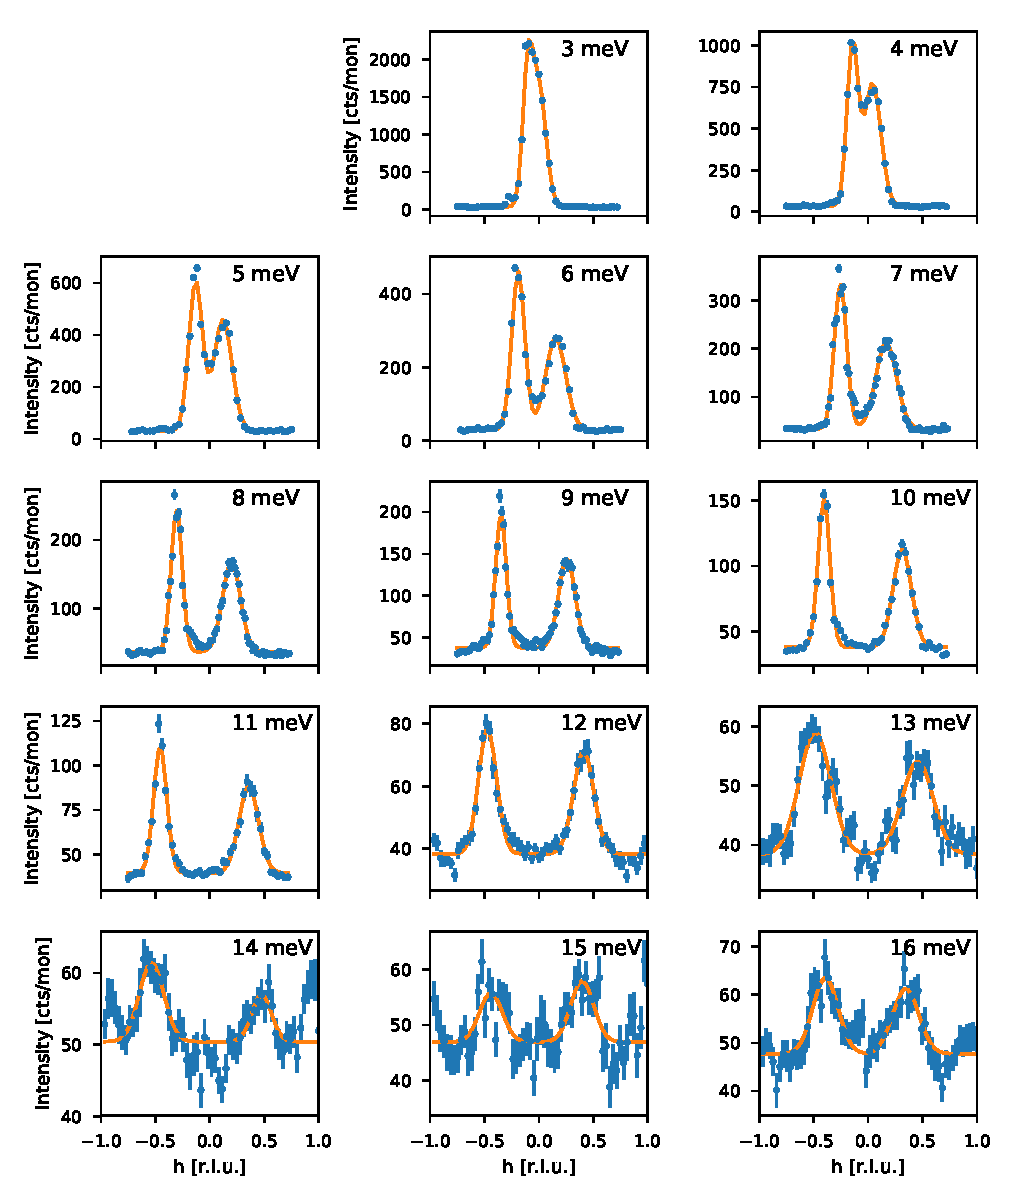
\includegraphics[width=\textwidth]{fig/lowen/fits_400T.pdf}
    \caption[400T flatcone raw data]{400T flatcone raw data}
    %label{fig:flatcone_phonons_400T_raw}    
\end{figure}

\begin{figure}
    \centering
    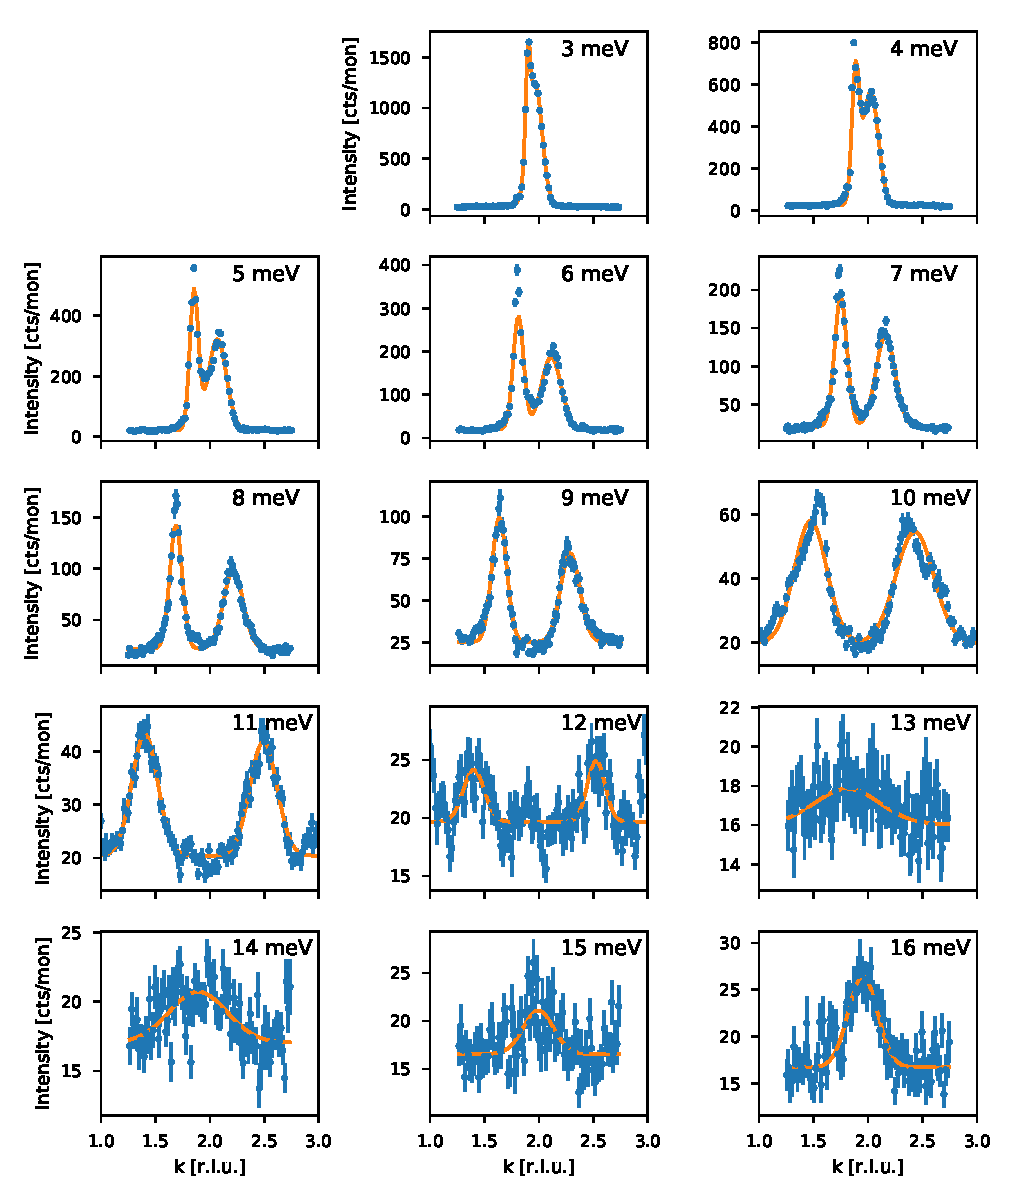
\includegraphics[width=\textwidth]{fig/lowen/fits_220T.pdf}
    \caption[220T flatcone raw data]{220T flatcone raw data}
    %\label{fig:flatcone_phonons_400T_raw}
\end{figure}

\begin{figure}
    \centering
    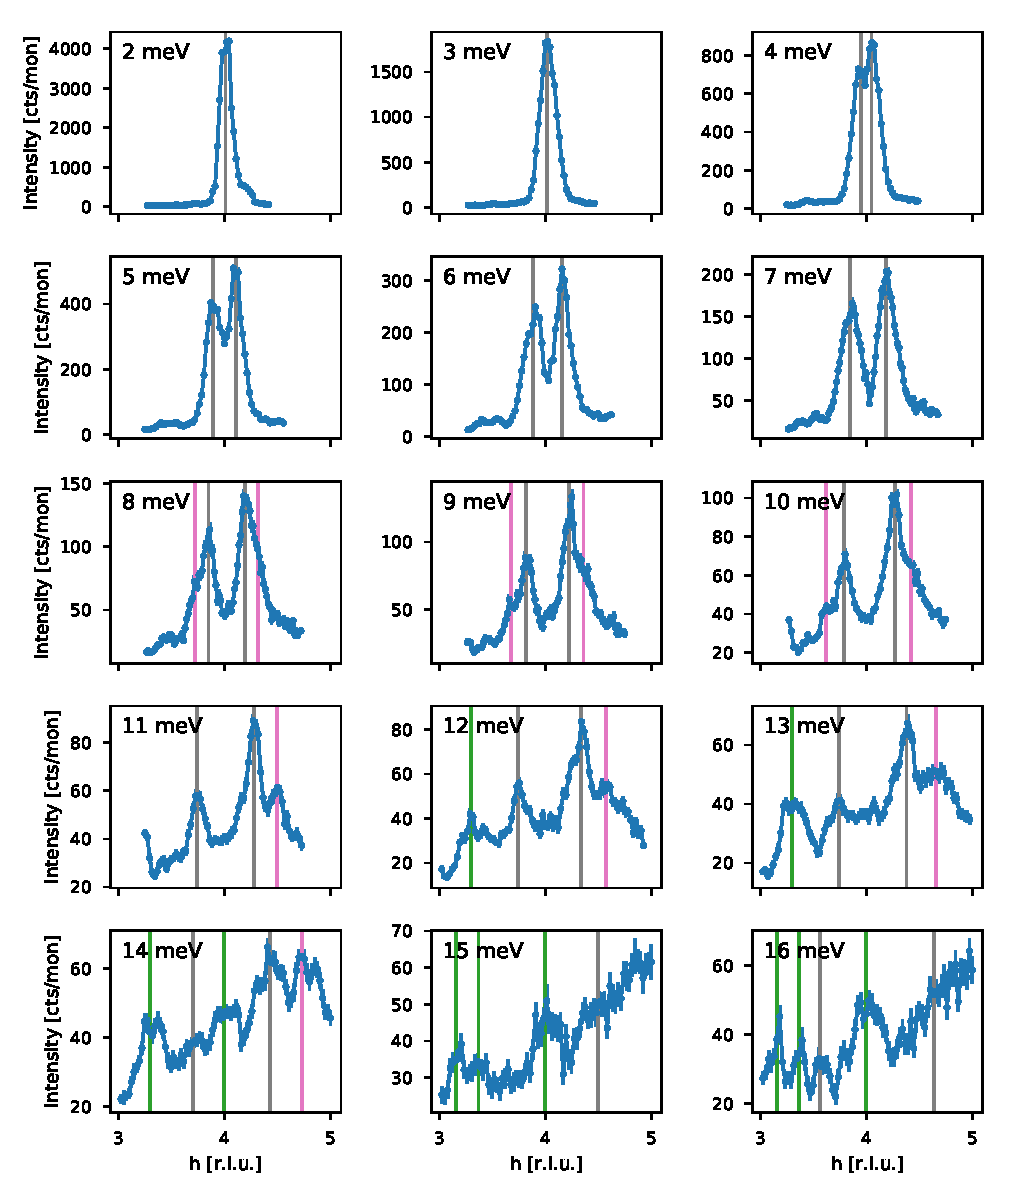
\includegraphics[width=\textwidth]{fig/lowen/fits_400L.pdf}
    \caption[400L flatcone raw data]{400L flatcone raw data}
    %\label{fig:flatcone_phonons_400L_raw}    
\end{figure}

\begin{figure}
    \centering
    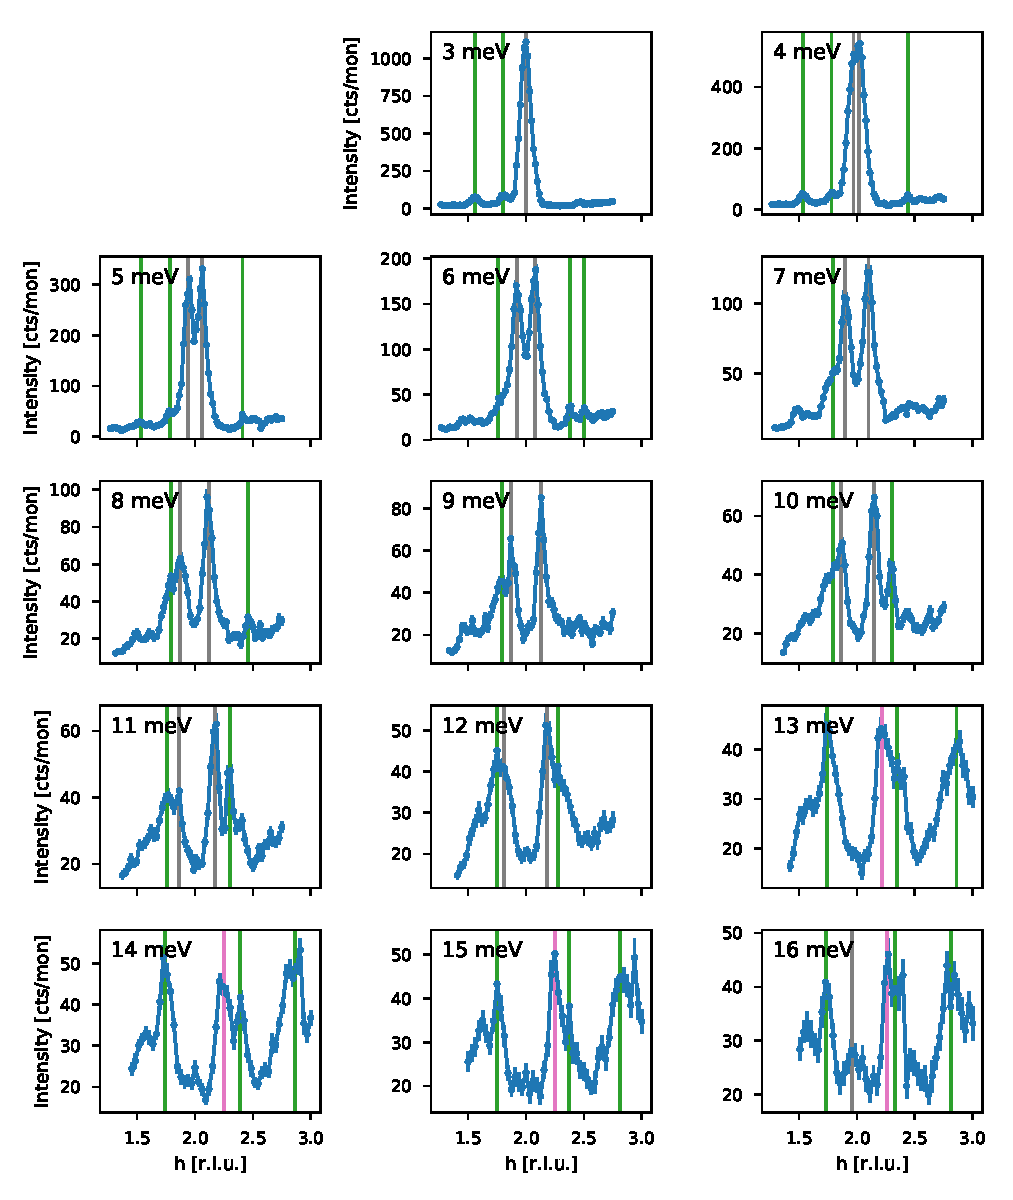
\includegraphics[width=\textwidth]{fig/lowen/fits_220L.pdf}
    \caption[220L flatcone raw data]{220L flatcone raw data}
    %\label{fig:flatcone_phonons_220L_raw}    
\end{figure}

\begin{figure}[]
    \centering
    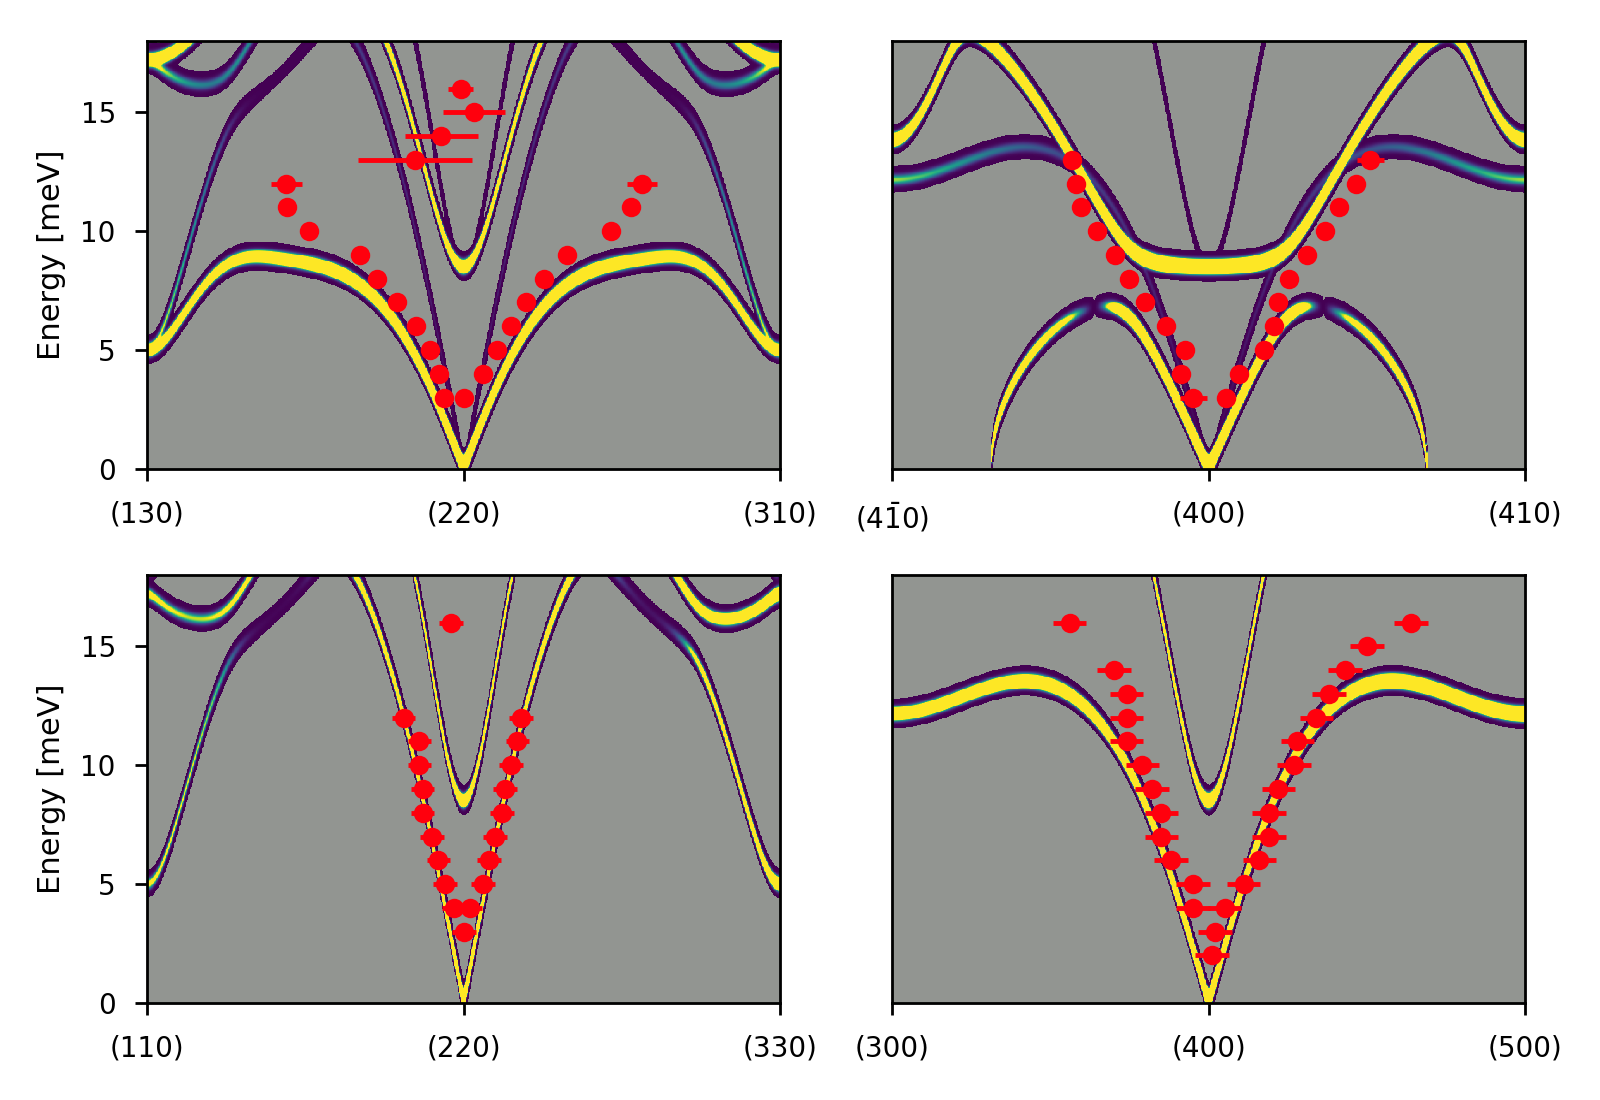
\includegraphics[width=\textwidth]{fig/lowen/flatcone_fits_simulation_htt_afm.png}
    \caption[Flatcone dispersion and neutron weighted simulation data]{Flatcone dispersion and neutron weighted simulation data. HTT AFM simulation data.}
    %\label{fig:flatcone_phonons_dispersion_simulation}
\end{figure}

\begin{figure}[]
    \centering
    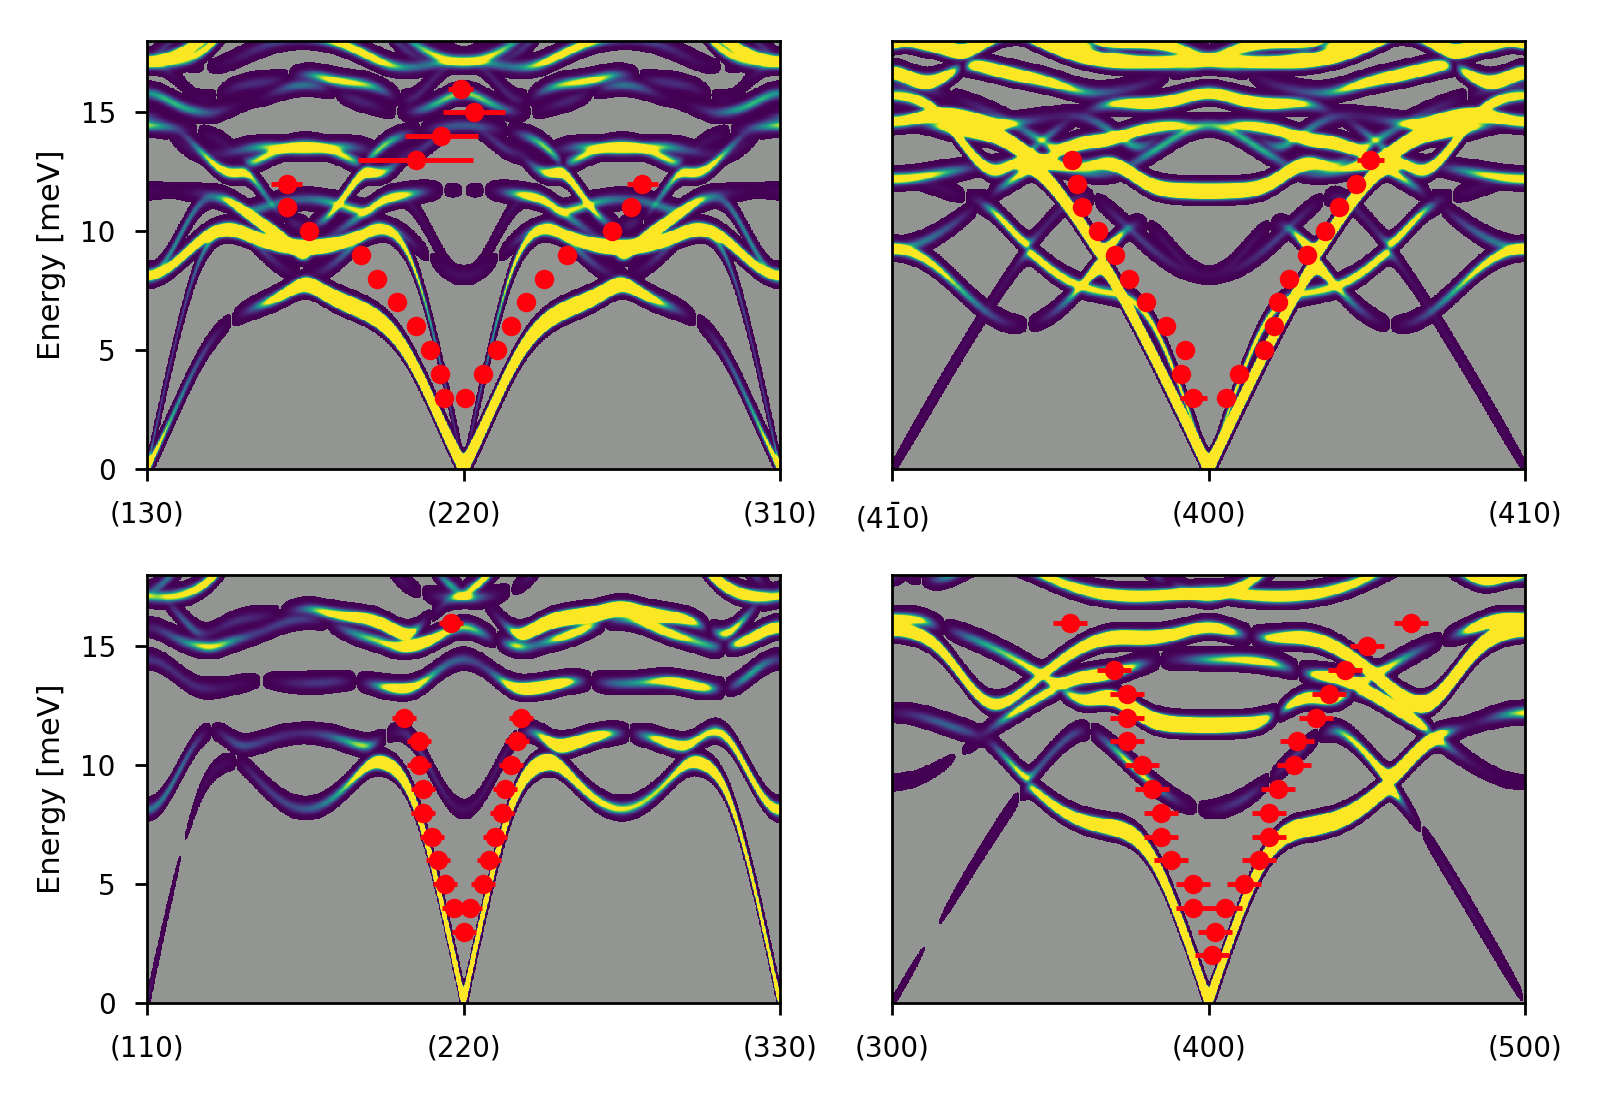
\includegraphics[width=\textwidth]{fig/lowen/flatcone_fits_simulation_ltt_afm.png}
    \caption[Flatcone dispersion and neutron weighted simulation data]{Flatcone dispersion and neutron weighted simulation data. LTT AFM simulation data.}
    %\label{fig:flatcone_phonons_dispersion_simulation}
\end{figure}

\begin{figure}[]
    \centering
    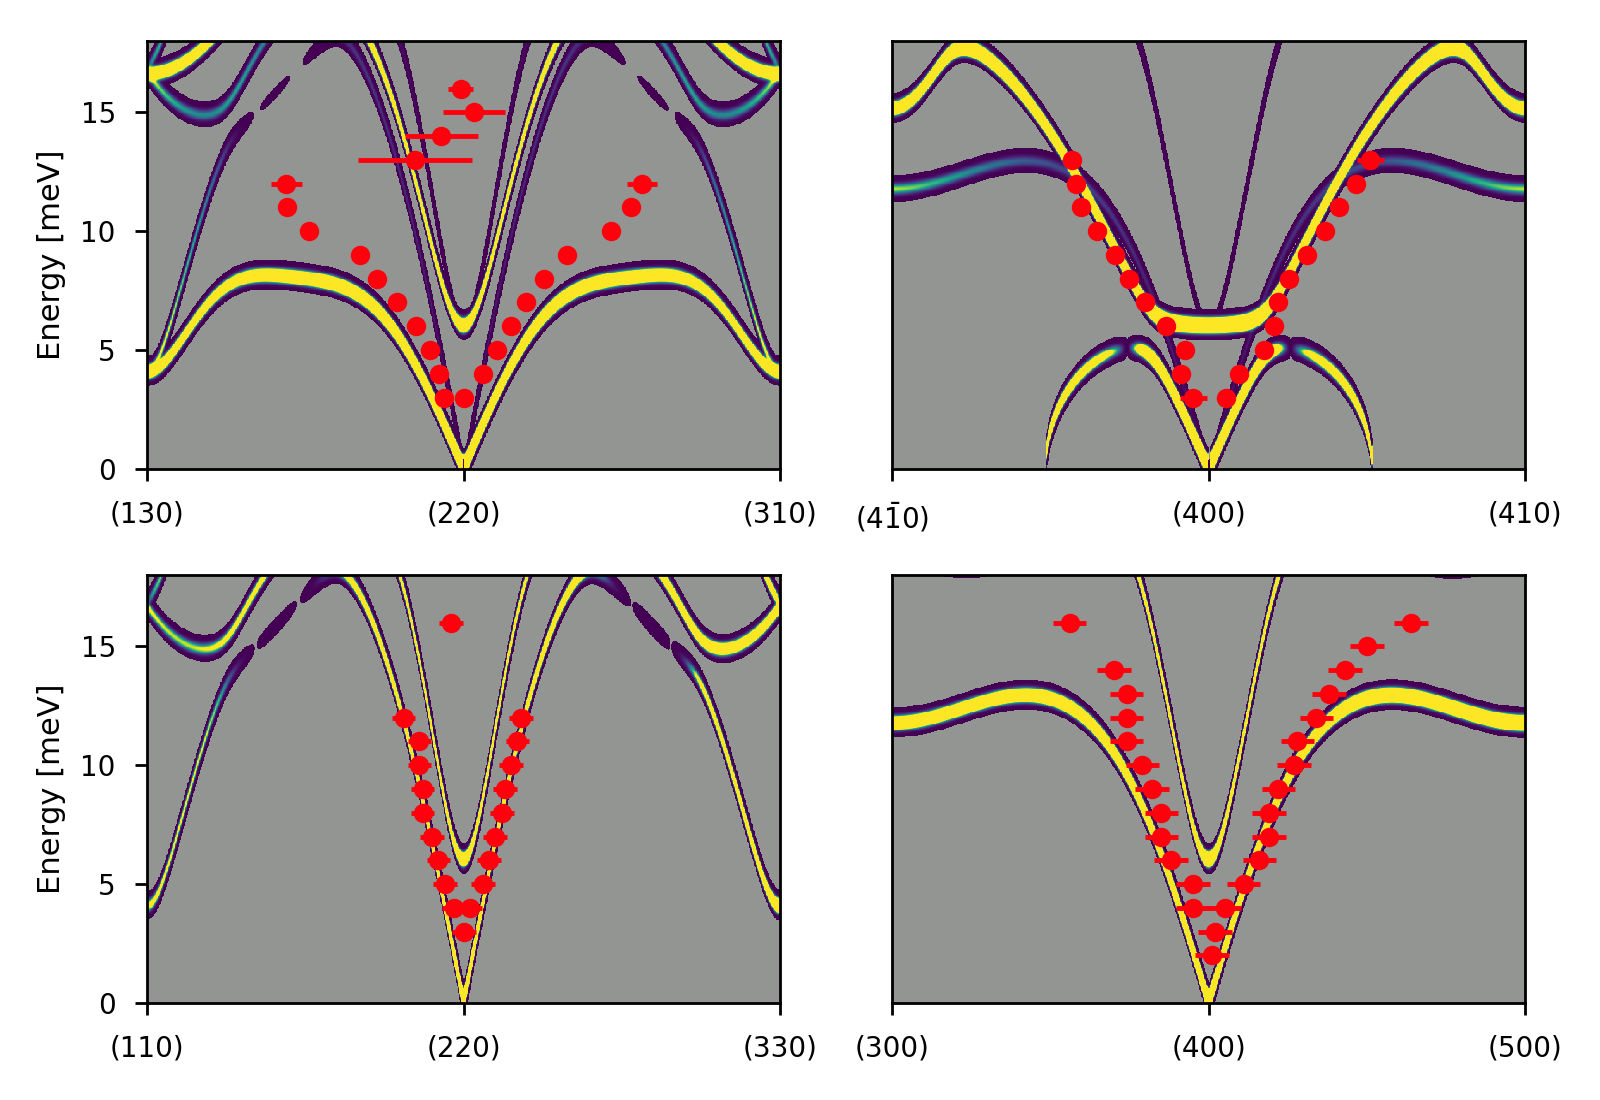
\includegraphics[width=\textwidth]{fig/lowen/flatcone_fits_simulation_htt_metal.png}
    \caption[Flatcone dispersion and neutron weighted simulation data]{Flatcone dispersion and neutron weighted simulation data. LTT AFM simulation data.}
    %\label{fig:flatcone_phonons_dispersion_simulation}
\end{figure}

\begin{figure}[]
    \centering
    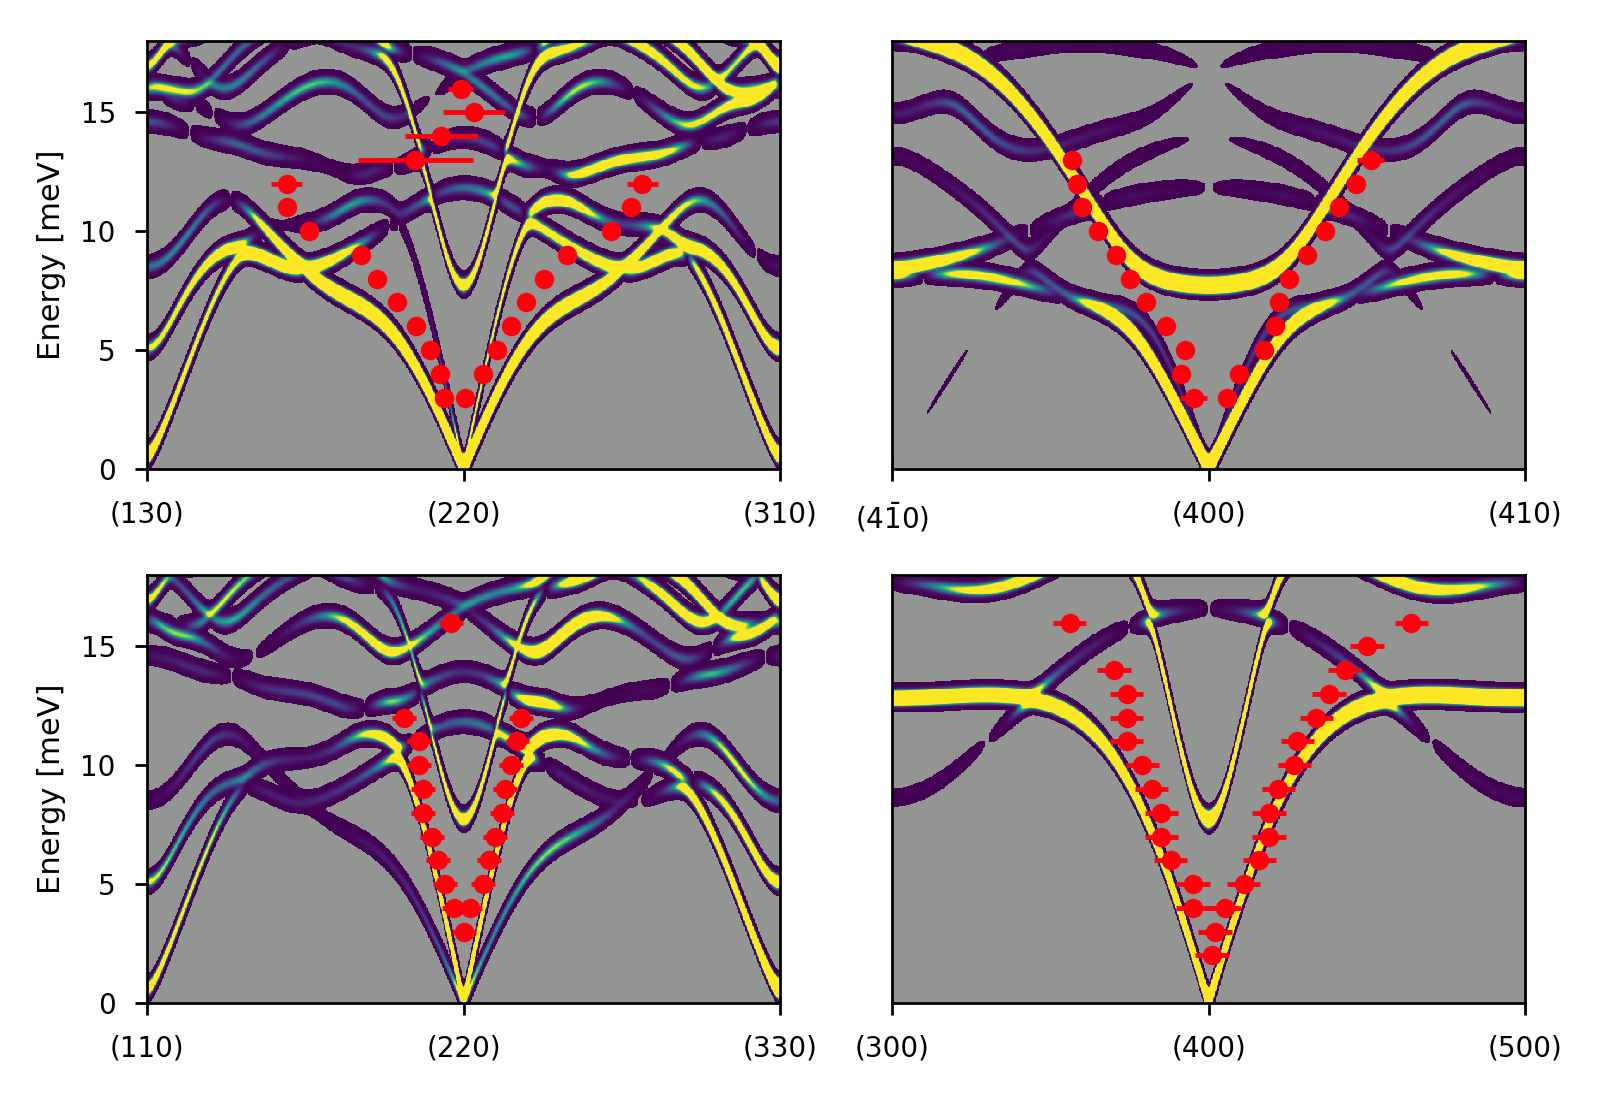
\includegraphics[width=\textwidth]{fig/lowen/flatcone_fits_simulation_lto_metal.png}
    \caption[Flatcone dispersion and neutron weighted simulation data]{Flatcone dispersion and neutron weighted simulation data. LTO metal simulation data.}
    %\label{fig:flatcone_phonons_dispersion_simulation}
\end{figure}

\begin{figure}[]
    \centering
    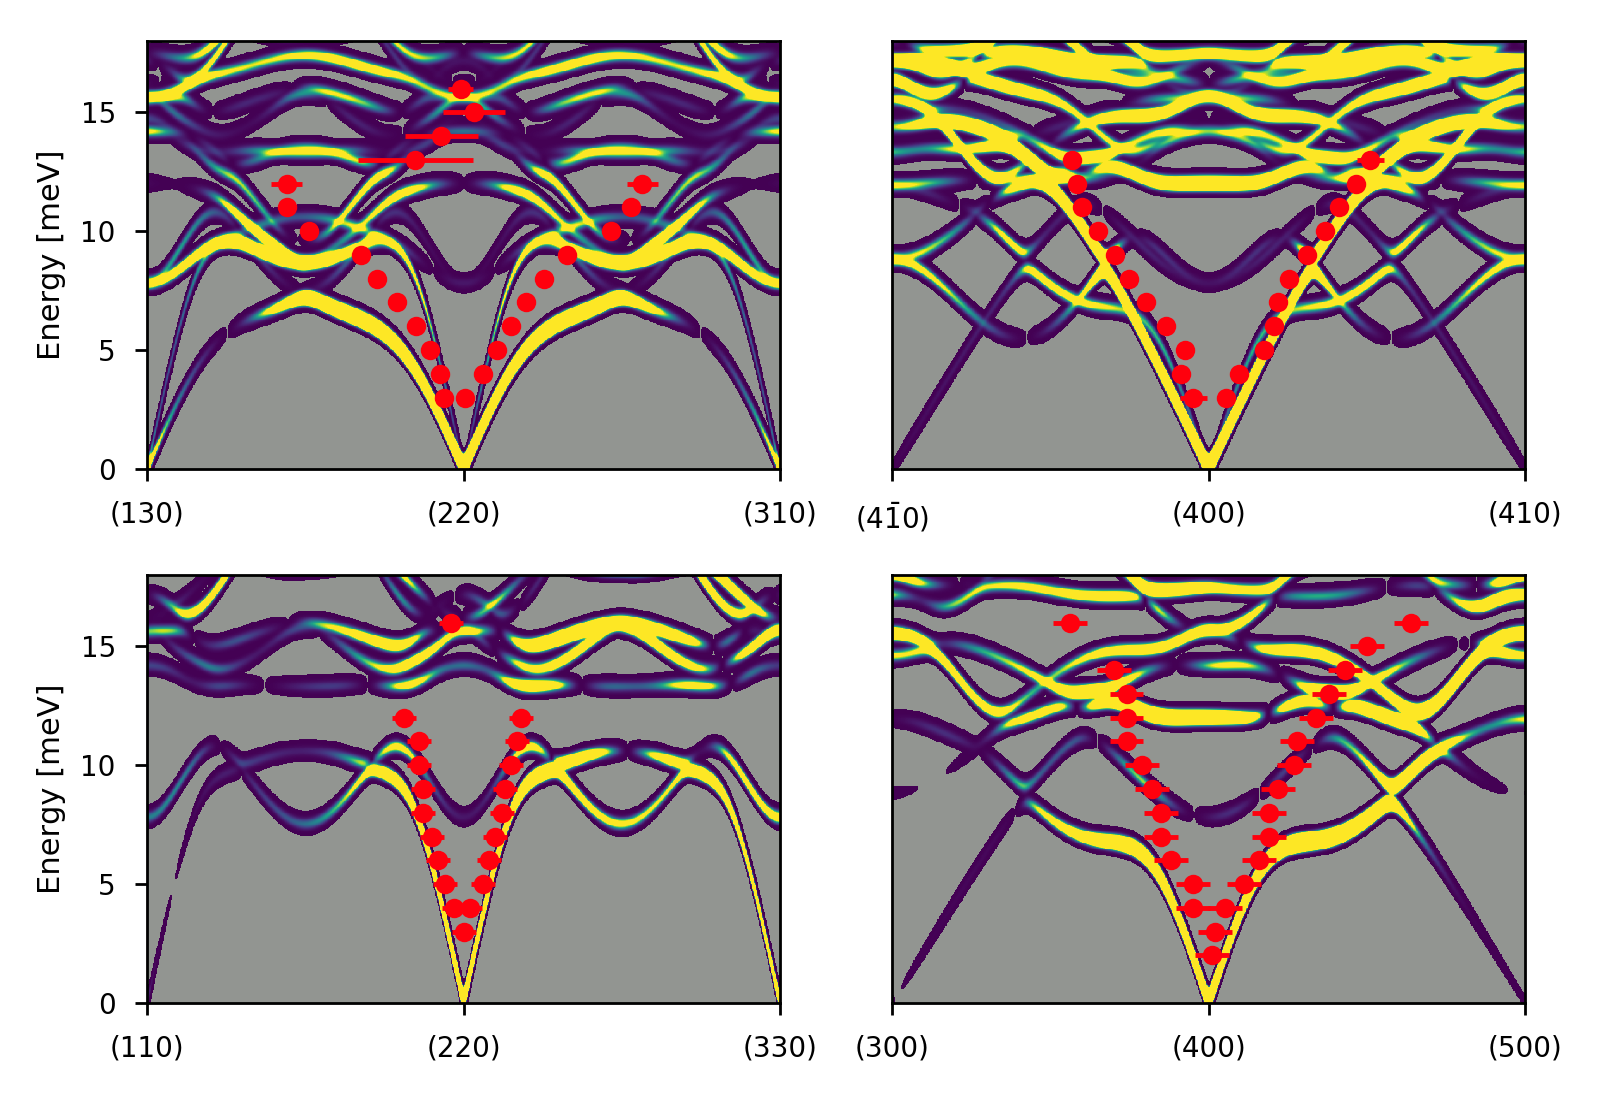
\includegraphics[width=\textwidth]{fig/lowen/flatcone_fits_simulation_ltt_metal.png}
    \caption[Flatcone dispersion and neutron weighted simulation data]{Flatcone dispersion and neutron weighted simulation data. LTT Metal simulation data.}
    %\label{fig:flatcone_phonons_dispersion_simulation}
\end{figure}

\chapter{Additional Phonon DOS plots}\label{app:pdos_plots}

\begin{figure}
    \centering
    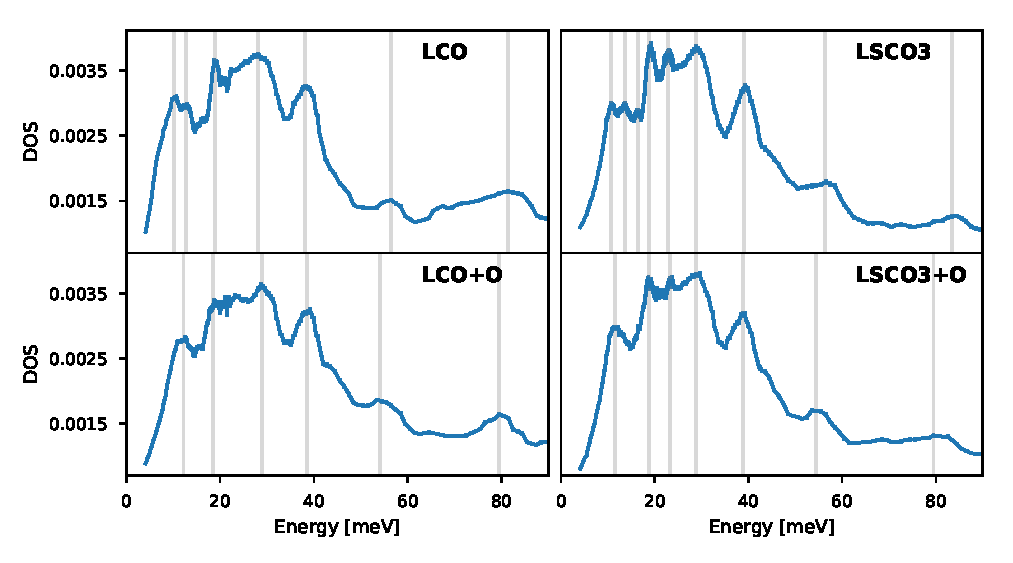
\includegraphics[width=\textwidth]{fig/gdos/in4_60K.pdf}
    \caption[gDOS at \SI{60}{\kelvin}]{GDOS at \SI{60}{\kelvin}}
    \label{fig:gdos_60k}
\end{figure}

\begin{figure}
    \centering
    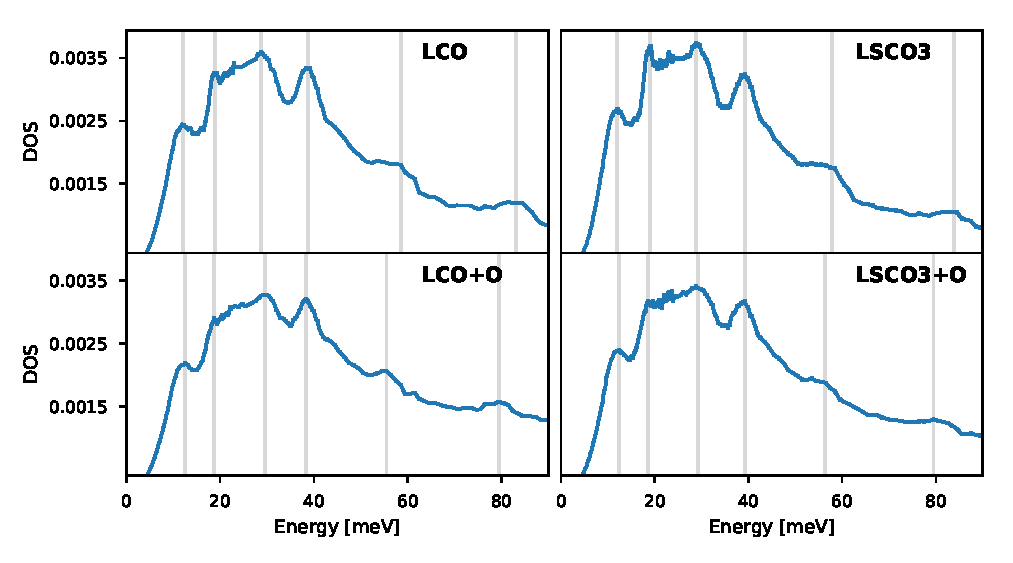
\includegraphics[width=\textwidth]{fig/gdos/in4_300K.pdf}
    \caption[gDOS at \SI{300}{\kelvin}]{GDOS at \SI{300}{\kelvin}}
    \label{fig:gdos_300k}
\end{figure}